\documentclass[9pt]{beamer}

\usepackage{amsmath}
\usepackage{amsfonts}
\usepackage{listings}

\setbeamersize{text margin left=5mm,text margin right=5mm}
\setlength{\leftmargini}{3mm}
\setlength{\leftmarginii}{3mm}
% \let\Tiny\tiny% http://tex.stackexchange.com/q/58087/5764

\newcommand{\vect}[1]{\mathbf{#1}}
\newcommand{\pder}[2][]{\frac{\partial#1}{\partial#2}}
\newcommand\RR{\mathbb R}


\begin{document}
\section{pnlss}
\label{sec:generate-data}

\begin{frame}<1>[label=pnlss]
  \begin{center}
    \visible<1>{Steps taken so far with PNLSS modeling}
  \end{center}
  \alert<1>{Generate data} \newline
  \alert<2>{Consistency} \newline
  \alert<3>{Nonparametric analysis} \newline
  \alert<4>{Parametric modeling}
\end{frame}

\begin{frame}{Avoid variable time step solvers}
  \begin{columns}
    \begin{column}{0.5\textwidth}
      To ensure periodicity, a fixed time step integrator is used
      \begin{itemize}
      \item Depending on forcing level, \texttt{ode45} at times gives nonperiodic
        output.
      \item Ex: low A; nonperiodic / high A; periodic\\
        guess: Low A allows for large step $\rightarrow$ interpolation destroys
        periodicity.
      \item Why RK5? Why not RK8/9/...?
        % https://scicomp.stackexchange.com/questions/25581/why-are-higher-order-runge-kutta-methods-not-used-more-often
        \begin{itemize}
        \item Higher order methods requires more function evaluations per step.
        \item Lower order have higher rounding errors.\\
        \item In celestial mechanics(oscillating over long time), at least RK8
          should be used. \url{https://doi.org/10.1007/BF00049361}
        \item Instead of increasing fs, RK8 might be used (next slide)
        \end{itemize}
      \item Alternative: 2-order Newmark-$\beta$; Not clear how to be used with
        benchmark4/5.
      \end{itemize}

    \end{column}
    \begin{column}{0.5\textwidth}  %%<--- here
      Example: Same system/forcing.\\ Upper: fixed step RK5, lower: ode45
      \begin{center}
        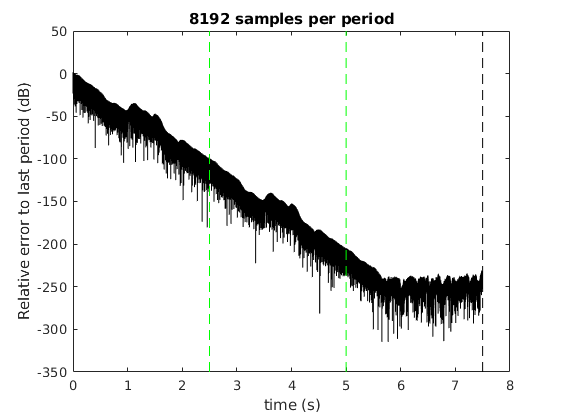
\includegraphics[width=0.9\textwidth]{fig/periodicity_ode5}
        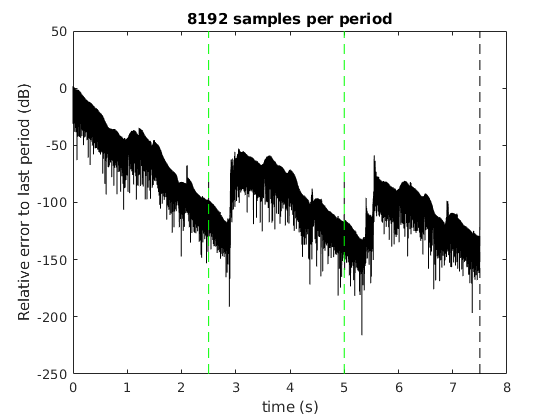
\includegraphics[width=0.9\textwidth]{fig/periodicity_ode45}
      \end{center}
    \end{column}
  \end{columns}
\end{frame}


\begin{frame}{Increase sampling frequency}
  \begin{columns}
    \begin{column}{0.5\textwidth}
      % \begingroup \small% \small in 11pt base font is 10pt
      To ensure numerical correct integration of highly nonlinear systems, we
      use a higher ``integration frequency'', fx \texttt{upsamp=20}
      \begin{itemize}
      \item Select integration \texttt{fsint} as multiple of desired \texttt{fs}.
        $fs_\text{int} =\text{upsamp} \cdot fs$
      \item downsample forcing, \texttt{u=u(1:upsamp:end)}. Since the Nyquist
        frequency for the downsampled fs is still above f2, the last excited
        frequency.
      \item decimate output. The nonlinear system might generate higher
        harmonics in the output: $y$ should be decimated; ie. first low-pass
        filtered and then downsampled to avoid aliasing.
      \end{itemize}
      % \endgroup
    \end{column}
    \begin{column}{0.5\textwidth}  %%<--- here
      Example: Same system/forcing.\\ Upper: $fs_\text{int} =\text{upsamp}\cdot fs$
      \begin{center}
        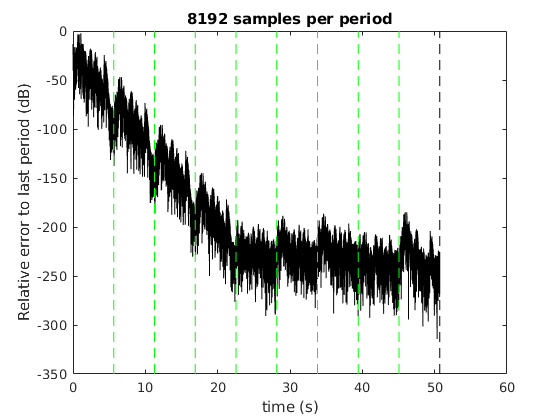
\includegraphics[width=0.9\textwidth]{fig/b1_A30_ms_full1_periodicity}
        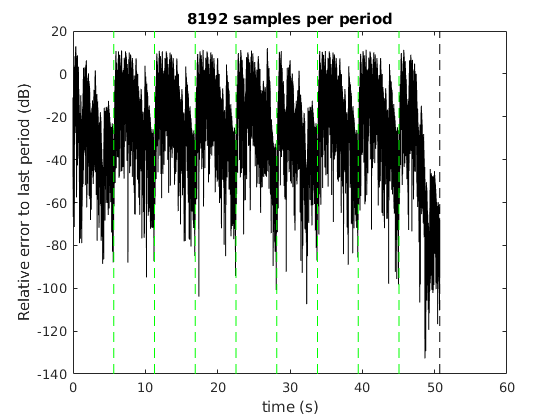
\includegraphics[width=0.9\textwidth]{fig/b1_A30_ms_full2_periodicity}
      \end{center}
    \end{column}
  \end{columns}
\end{frame}


\begin{frame}{Use RK8 - maybe}
  RK8 with fixed time step.
  \begin{itemize}
  \item RK8 steady state is reached after 3 periods. High $A$.
  \item RK5 with upsamp: SS after 4 periods (previous slide). High $A$.
  \item Not clear why different
  \item But BLA(angle) is not estimated properly for RK8 data. Low $A$\\
    Upper: RK8; lower: RK5
  \item ... but estimated PNLSS models are similar.
  \end{itemize}
  \begin{center}
    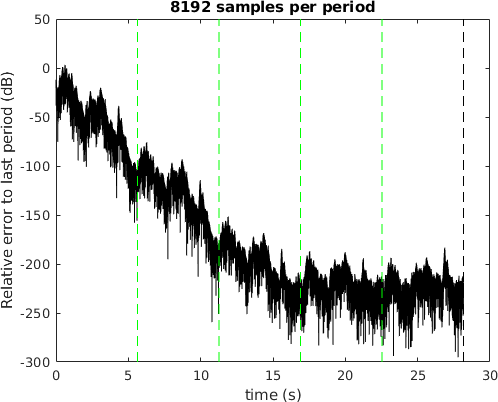
\includegraphics[width=0.45\textwidth]{fig/b1_A30_ode8_periodicity}
    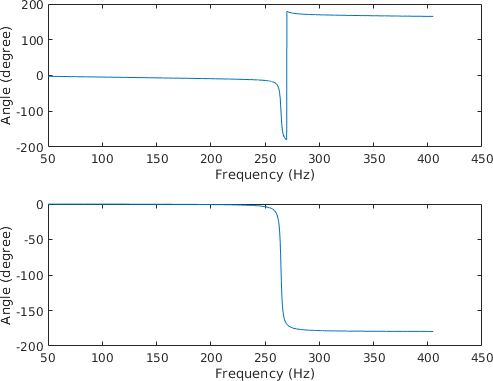
\includegraphics[width=0.45\textwidth]{fig/angle_rk8_rk5}
 \end{center}
\end{frame}

\againframe<2>{pnlss}


\begin{frame}{Discrete model}
  The EOM for the duffing oscillator in benchmark1 can be written as
  % see JJT p 115
  \begin{equation}
    \label{eq:duffing}
    \ddot y + 2\beta\omega_0\dot y + \omega_0^2 y + \gamma y^3 = q\cos(\Omega t)
  \end{equation}

  Using the state vector $\vect u = [y\,\dot y]^T $, the duffing eq. is written in state space
  \begin{equation}
    \label{eq:duffing_ss_ct}
    \left\lbrace
      \begin{aligned}
        \dot x_1(t) &= x_2(t) \\
        \dot x_2(t) &= u(t) - 2\beta\omega_0x_2(t) - \omega_0^2x_1 - \gamma x_1^3
      \end{aligned}
    \right.
  \end{equation}
  where $u(t)=q\cos(\Omega t)$. The continuous-time model is converted into
  discrete-time using a forward Euler discretization, ie. $\dot x =
  \frac{x(t+h)-x(t)}{h}$

  \begin{equation}
    \label{eq:duffing_ss_dt}
    \left\lbrace
      \begin{aligned}
        \dot{\vect x(t+h)} &=
        \begin{bmatrix}
          1 & h \\ -\omega_0^2h & 1-\beta\omega_2h
        \end{bmatrix} \vect x(t) +
        \begin{bmatrix}
          0 \\ h
        \end{bmatrix} u(t) +
        \begin{bmatrix}
          0 \\ -\gamma h
        \end{bmatrix} x_2^3(t) \\
        y(t) &=
        \begin{bmatrix}
          1 & 0
        \end{bmatrix} \vect x(t)
      \end{aligned}
    \right.
  \end{equation}

  Compare this to the general PNLSS form
  \begin{equation}
    \label{eq:pnlss}
    \left\lbrace
      \begin{aligned}
        \vect x(t+1) &= \vect A \vect x(t) + \vect B \vect u(t) + \vect E \vect g(x,u) \\
        \vect y(t) &= \vect C \vect x(t) + \vect D \vect u(t) + \vect F \vect h(x,u)
      \end{aligned}
    \right.
  \end{equation}
  This is only a good approximation for small $h$ due to the simplicity of the
  differentiation rule.
\end{frame}


\begin{frame}{Approaches for comparing the linear part of PNLSS(A,B,C,D)}

  PNLSS identify discrete time state space matrices. $\vect A_k$ and $\vect
  B_k$(discrete time) is converted to continuous time (no conversion needed for
  C and D). We assume a correct identified nonlinear model is needed for the
  linear parameters to be correct.

  \begin{itemize}
  \item SS models are not unique. Use a similarity transform $ \vect x = \vect T
    \hat {\vect x}$ (linear change of state variable coordinates) to get
    physical coordinates $\vect x$.\footnotemark[1]
    \begin{equation}
      \label{eq:similarity_transform}
      \vect A = \vect T \hat {\vect A} \ \vect T^{-1}, \quad
      \vect B = \vect T \hat {\vect B}, \quad
      \vect C = \hat {\vect C} \vect T^{-1}, \quad
      \vect D = \hat {\vect D}, \quad
      \vect T =
      \begin{bmatrix}
        \hat {\vect C} \\  \hat {\vect C}  \hat {\vect A}
      \end{bmatrix}
    \end{equation}
  \item Compare invariant parameters.
    \begin{itemize}
    \item The transfer function $\vect G(z) = \vect D + \vect C(z \vect I -
      \vect A)^{-1}\vect B$.\\
    \item or eigenvalues of $\vect A$(poles)
    \end{itemize}
  \end{itemize}


  \footnotetext[1]{Etienne Gourc, J.P. Noël, et.al:
    Obtaining Nonlinear Frequency Responses from Broadband Testing
    \url{https://orbi.uliege.be/bitstream/2268/190671/1/294_gou.pdf}}
\end{frame}


\begin{frame}{Compare nonlinear model with true system.}
  \begin{itemize}
  \item Compute RMS error of the PNLSS simulated signal compared with the 'true'
    simulated system.
  \item Simulate the PNLSS model with NLvib; obtaining a frequency response directly comparable
  \item We are not aware of any way to compare the identified E/F
    matrices(coefficients of the nonlinear state-dependent polynomials) with the
    true system.
  \end{itemize}
\end{frame}


\begin{frame}[fragile]{general PNLSS settings around 1 mode}
  Ensure that there is no modal interaction by setting the multisine amplitude
  lower than the level where we expect tongues and ensuring high
  enough damping of higher modes.\\
  For benchmark 1-3 (polynomial nl):

\begin{lstlisting}[language=matlab]
    n = 2;
    whichtermsx = 'statesonly';
    whichtermsy = 'empty';
    nx = [3]    % benchmark 1/2
    nx = [2,3]  % benchmark 3
\end{lstlisting}
  Nonlinear monomials
  \begin{itemize}
  \item[$nx = [2,3]$]: $x_1^2,x_1x_2,x_2^2$, $x_1^3,x_1^2x_2,x_1x_2^2,x_2^3$ $\rightarrow$ 23
    parameters to estimate
  \item[$nx = [3]$]: $x_1^3,x_1^2x_2,x_1x_2^2,x_2^3$ $\rightarrow$ 17 parameters
  \end{itemize}


\end{frame}


\againframe<3>{pnlss}


\begin{frame}{Characterization of nonlinearity}
  Use random-odd multisine. Only odd frequency lines are excited. For each group
  of four lines, one is randomly set to zero.
  \begin{equation}
    \label{eq:multisine}
    u(t) = U \sum_{n=1}^N A_n \sin(2\pi nf_0t + \phi) / \textstyle \sqrt{\sum_n A_n}
  \end{equation}
  Normalized to ensure constant power as the number of included harmonics $N$ is
  varied. $A_n$ is a boolean, $f_0$ frequency resolution(or fundamental
  frequency). Number of periods is chosen by end time $t_2=P/f_0$.

  A general conclusion: The only way to increase the freq. resolution is to
  increase the measurement time. Increasing the sampling frequency does not
  help.

  %\begin{column}{0.5\textwidth}  %%<--- here
    \begin{center}
      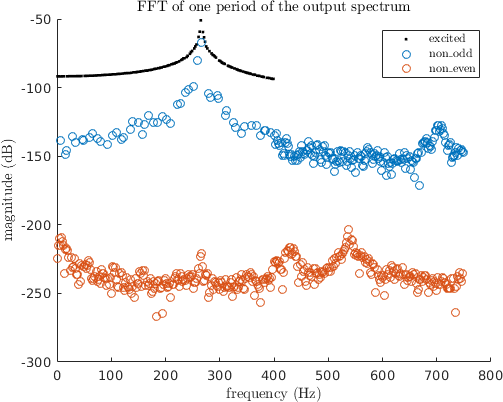
\includegraphics[width=0.45\textwidth]{fig/ms_nl_detection_b2}
      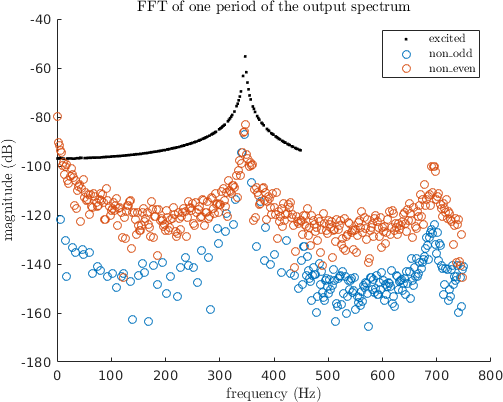
\includegraphics[width=0.45\textwidth]{fig/ms_nl_detection_b3}\\
      left: straight beam; right: curved beam
    \end{center}
  %\end{column}
\end{frame}


\begin{frame}{Estimating distortion levels}
  \begin{columns}
    \begin{column}{0.5\textwidth}
      Use full multisine. Average over periods and realizations to estimate noise
      and nonlinear distortion $\rightarrow$ is NL-model necessary?\\

      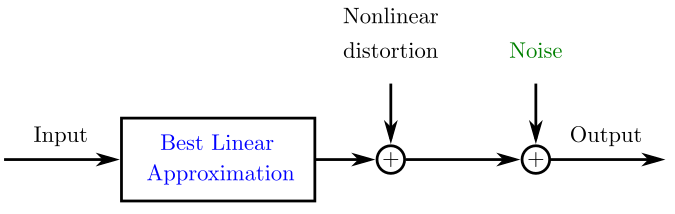
\includegraphics[width=0.99\textwidth]{fig/bla_nldistort}

      \vspace*{5mm}

      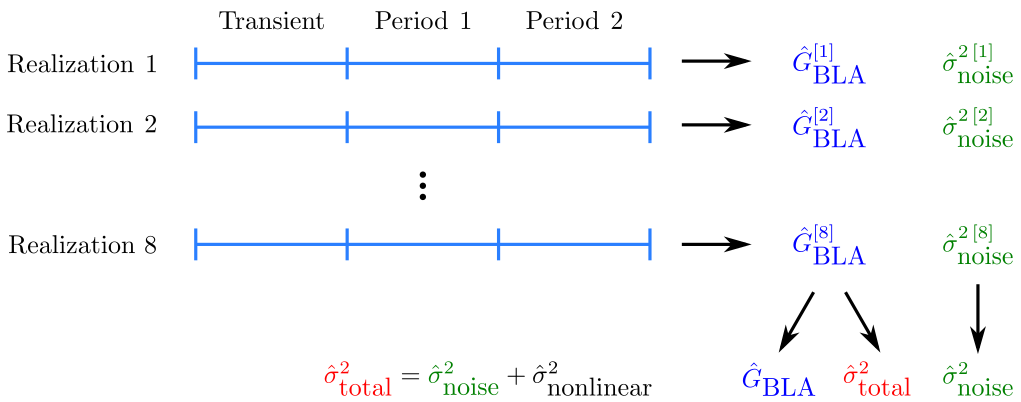
\includegraphics[width=0.99\textwidth]{fig/ms_nldistort}
    \end{column}
    \begin{column}{0.5\textwidth}
      \vspace{-5mm}

      Increasing NL distortion with increasing A
      \vspace{-1mm}
      \begin{center}
        upper: $A=1$; lower $A=30$\\
        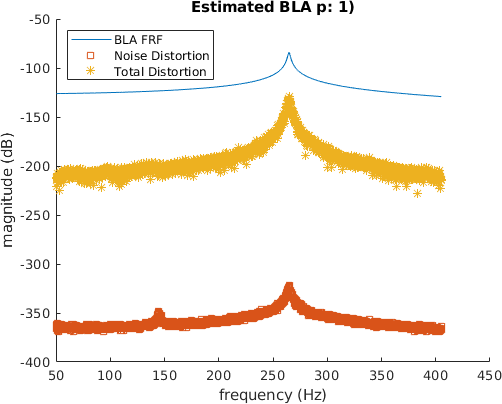
\includegraphics[width=0.75\textwidth]{fig/b1_A1_ms_full_bla}
        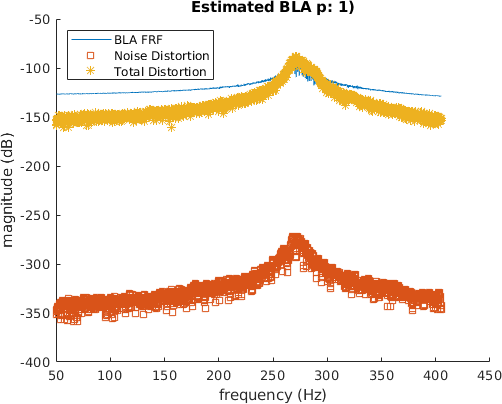
\includegraphics[width=0.75\textwidth]{fig/b1_A30_ms_full_bla}
      \end{center}
    \end{column}
  \end{columns}
  \tiny{Note: dB for power: $L_p=10\log_{10}(P)$. dB for field quantity:
    $L_F=10\log_{10}(F^2)$. Thus when comparing distortion(variance,
    proportional to power) with $|G|$, do either (matlab pseudo-syntax)
    (Also remember to multiply distortion with number of realizations):\\
    \texttt{plot(freq,[db(abs(G)), db(var*R,'power')])} or
    \texttt{plot(freq,[db(abs(G)), db(sqrt(var*R))])}}.
\end{frame}


\againframe<4>{pnlss}


\begin{frame}{Subspace model}
  \begin{itemize}
  \item Linear model of good quality\\
    Model error and standard deviation of BLA coincides
  \item Error seems to increase around 400 Hz.\\
    First thought: Maybe a second order discrete model is insufficient to model
    the continuous system. But third order shows same behavior
  \end{itemize}
  \begin{center}
    left: BLA and subspace($n=2$); right: cost function for different subspace
    models
    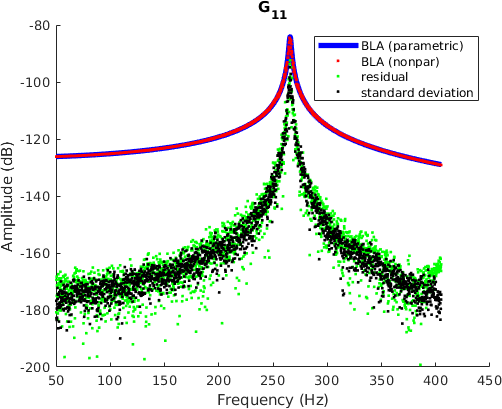
\includegraphics[width=0.45\textwidth]{fig/b1_A10_ms_full_subspace_n2}
    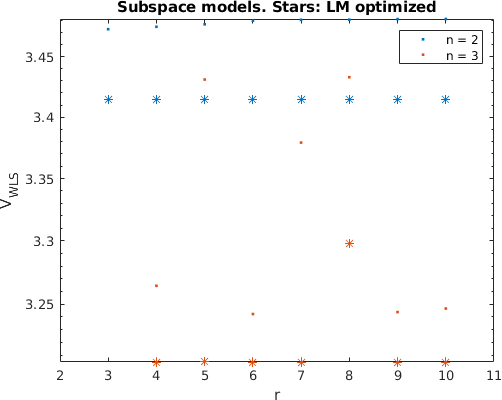
\includegraphics[width=0.45\textwidth]{fig/b1_A10_ms_full_sub_cost}
  \end{center}
\end{frame}


\begin{frame}{Full optimized model}
  \begin{itemize}
  \item Linear error significant around resonance(larger amplitudes)
  \item PNLSS RMS error decreased 3 orders of magnitude
  \item Not much difference in $\omega_0$ or $\zeta$.
  \item For fully correct model, pnlss error should be equal to noise floor (no
    noise, ie. error should be as low as integration precision).\\
    Here: 80 dB $\rightarrow$ $10^{-4}$.
  \end{itemize}

  \begin{center}
  \begin{tabular}{l|r|r|r}
    & $\omega_0$ Hz & $\zeta$ \% & \small{RMS error (new data)}\\
    \hline
    duffing & 264.72 & 0.38 &\\
    linear & 265.76 & 0.37  & 1.64$\cdot 10^{-5}$ \\
    pnlss & 264.72 & 0.38 & 7.46$\cdot 10^{-8}$
  \end{tabular}
  \vspace{2mm}

    left: convergence; right: Error on new data\\
    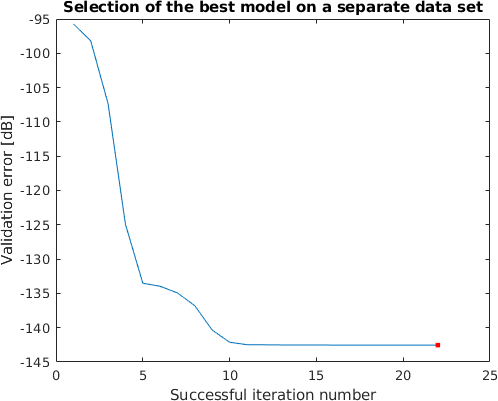
\includegraphics[width=0.45\textwidth]{fig/b1_A10_ms_full_convergence}
    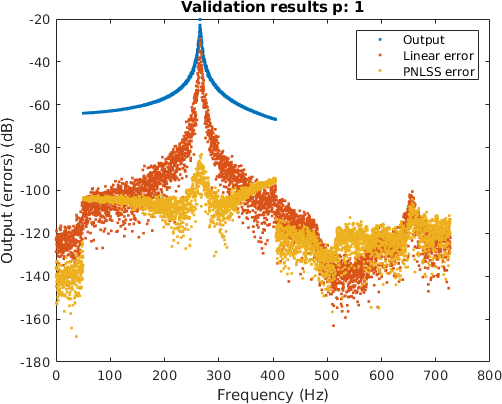
\includegraphics[width=0.45\textwidth]{fig/b1_A10_ms_full_val_err_p1}
  \end{center}
\end{frame}


\begin{frame}[fragile]{Noise}
  \begin{itemize}
  \item SNR?
  \item Type/color?
  \end{itemize}

  \begin{lstlisting}
    noise = 1e-3*std(y(:,end,end))*randn(size(y));
    % Do some filtering
    noise(1:end-1,:,:) = noise(1:end-1,:,:) + noise(2:end,:,:);
  \end{lstlisting}
  \begin{center}
  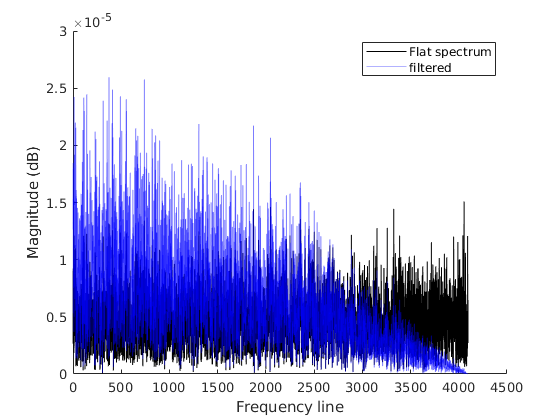
\includegraphics[width=0.55\textwidth]{fig/noise}
\end{center}
\end{frame}


% e_est_lin:	 1.860e-05	 e_est_nl:	 7.570e-08
% e_val_lin:	 1.639e-05	 e_val_nl:	 7.465e-08
% e_test_lin:	 1.530e-05	 e_test_nl:	 4.152e-06

% Nat freq 264.72, 264.72,  Hz.
% damping 0.003798

% 264.7179


% Identified Modal Parameters
% Nat freq 265.76, 265.76,  Hz.
% damping 0.0037382, 0.0037382,

\end{document}

%%% Local Variables:
%%% mode: latex
%%% coding: utf-8-unix
%%% TeX-engine: luatex
%%% magic-latex-enable-block-highlight: nil
%%% End: